\documentclass[conf]{new-aiaa}
%\documentclass[journal]{new-aiaa} for journal papers
\usepackage[utf8]{inputenc}

\usepackage{graphicx}
\usepackage{amsmath}
\usepackage[version=4]{mhchem}
\usepackage{siunitx}
\usepackage{longtable,tabularx}
\setlength\LTleft{0pt} 

\title{AE 5335 Midterm}
\author{Riley J. Kyle} 

\begin{document}

\maketitle



\clearpage

\begin{figure}[hbt!]
    \centering
    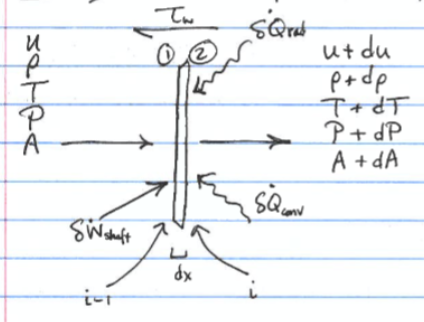
\includegraphics[width=0.4\textwidth]{images/quasi1D.png}
    \caption{Quasi 1D flow}
\end{figure}

\section{Methodology}


For this assignment a code was developed to integrate the quasi-1D flow equations using the callorically perfect gas assumption.
The equations of state are:

\begin{equation}
    \frac{d\rho}{\rho} + \frac{du}{u} + \frac{dA}{A} = 0
\end{equation}

\begin{equation}
    \frac{dP}{\rho} + u du = \frac{-\tau_w c dx}{\rho A} + \eta \delta w_{shaft}
\end{equation}

\begin{equation}
    C_p dT + u du = \delta q + \delta w_{shaft}
\end{equation}

\begin{equation}
    \frac{dP}{P} = \frac{d\rho}{\rho} + \frac{dT}{T}
\end{equation}

In this current form we are left with a system of 4 equations with 4 unknowns which can be solved for using a root solving algorithm.
However, since root solvers themselves can be computationally expensive and introduce numerical additional numerical errors an additional step was made.
The system of equations shown above was reduced algebraically to a single equation with one unknown.
The variable that was solved for was $du$ due to its presence in the continuity, momentum, and energy equations.


\begin{equation}
    du = -
    \frac{\frac{\rho}{P}\left(\eta dw - \frac{\tau_w c dx}{\rho A}\right)
    - \frac{dq+dw}{Cp T} + \frac{dA}{A}}
    {\frac{1}{u}-\frac{u}{R T} + \frac{u}{Cp T}}
\end{equation}

The code itself will take the following inputs: an array with the velocity, temperature, and pressure.;
A function defining the area of the stream tube with respect to x;
length of the stream tube;
name of the working fluid;
number of iterations;
work per mass through the stream tube;
heat per mass through the stream tube;
skin friction coefficient;
work efficiency;
and wall temperature. 


After entering these inputs and pre-generating arrays, equation 5 was used to solve for $du$. 
This was then entered into equations 2 and 3 to find $dP$ and $dT$.
This was then plugged into equation 4 to solve for $d\rho$. 
$dw$ is defined as the total work divided by the number of axial steps and $dq$ for circular ducts is defined as:

\begin{equation}
    dq = dq_{conv} + dq_{rad} =  
    2 C_p C_f \left(T_w - T_t\right)\frac{dx}{D} + \frac{q}{N}
\end{equation}

Using this methodology, calculating the fluid dynamics through a stream tube using the quasi 1D approach with 1 million steps takes 4.9 seconds.
As shown in the results, it is able to do this while only having small numerical differences with the analytical solution.
\pagebreak 

\section*{Case 1}


\section*{Case 2}



\section*{Case 3}



\section*{Case 4}



\section*{Case 5}



\section*{Case 6}



\section*{Case 7}


\end{document}